% !TEX program = pdflatex
\documentclass[3p,11pt]{elsarticle}
\usepackage{amsmath,amssymb}
\usepackage{array}
\usepackage{booktabs}
\usepackage[tableposition=top]{caption}
\usepackage{graphicx}
\usepackage{url}
\urlstyle{same}
\usepackage[hidelinks]{hyperref}
\emergencystretch=3em
% first-page footer: the page number alone
\makeatletter
\def\ps@pprintTitle{\let\@oddhead\@empty\let\@evenhead\@empty
  \def\@oddfoot{\hfil\thepage\hfil}\let\@evenfoot\@oddfoot}
\makeatother

% ---- notation ---------------------------------------------------------------
\newcommand{\kms}{km\,s$^{-1}$}
\newcommand{\ms}{m\,s$^{-1}$}
\newcommand{\Msun}{M$_\odot$}
\newcommand{\Rsun}{R$_\odot$}
\newcommand{\Lsun}{L$_\odot$}
\newcommand{\Mearth}{M$_\oplus$}

\begin{document}

\begin{frontmatter}

\title{Evidence for a planet of 30 Earth masses on a 37-day orbit around HD\,125881, in public HARPS
velocities}

\author{Charles C. Norton}

\begin{abstract}
HD\,125881 (HIP\,70459) is a G2 dwarf of 1.02\,\Msun\ at 36.2\,pc, about 6\,Gyr old and magnetically
quiet. Its public HARPS velocities, from 52 nights between 2004 and 2013, carry a Keplerian signal at
37.02\,d with a semi-amplitude of 5.7\,\ms, which a planet of at least 30\,\Mearth\ at 0.22\,au would
make. The signal stands in three reductions of the spectra, SERVAL's velocities, the HARPS pipeline's
and line-by-line velocities measured here, at false-alarm levels of $2\times10^{-7}$, $3\times10^{-7}$
and $8\times10^{-6}$, and no activity indicator has power at the period. Twenty-seven of the
nights fall within one month of 2013, shorter than the period, and hold most of the signal's weight:
within that month the velocities vary smoothly at a false-alarm level of $10^{-9}$. The 25 nights of
2004 to 2012 do not find the signal on their own, and fitted at the orbit's period and phase they
give $4.9 \pm 1.0$\,\ms. The one-year alias at 33.6\,d fits worse by 12.6 in log-likelihood; the
other, at 41.2\,d, fits worse by 2.9, and one simulation of the observing window in three hundred
with the planet there reproduces the observed periodogram. TESS observed the predicted conjunction of
2019 May entirely, where it excludes a central transit of a planet larger than 3.3 Earth radii, and
those of 2021 May and 2026 February in part. Velocities spread over two or three months would confirm
the planet and its period.
\end{abstract}

\begin{keyword}
Techniques: radial velocities \sep Planets and satellites: detection \sep Stars: individual: HD\,125881
\end{keyword}

\end{frontmatter}

\section{Introduction}\label{sec:intro}

Planets of a few tens of Earth masses on orbits of weeks, between Neptune and Saturn in mass, are
found less often by radial-velocity surveys of Sun-like stars than the smaller planets on such
orbits~\cite{Howard2010}. HARPS-RVBank~\cite{Trifonov2020} recomputed every public HARPS velocity with
SERVAL~\cite{Zechmeister2018}, corrected the instrument's nightly zero points and attached each
spectrum's activity indicators, so that a star's whole record can be read at once, and DACE serves the
HARPS pipeline's own velocities of the same spectra.

HD\,125881 is one of the stars that record holds. HARPS observed it on 52 nights between 2004 and
2013, and no planet has been reported around it. Its velocities carry a signal that a planet of at
least 30 Earth masses on a 37-day orbit would make, HD\,125881\,b. Section~\ref{sec:data} describes the
data, Section~\ref{sec:star} the star, Section~\ref{sec:signal} the signal, its sampling and its
aliases, Section~\ref{sec:tests} the tests against the instrument and stellar activity,
Section~\ref{sec:orbit} the orbit and the mass, Section~\ref{sec:tess} TESS's photometry, and
Section~\ref{sec:discussion} what the case rests on.

\section{Data}\label{sec:data}

HARPS-RVBank holds 76 velocities of HD\,125881 from 52 nights between 2004 February 25 and 2013 May 3,
all before HARPS's fibre upgrade of 2015 June~\cite{LoCurto2015}, with a median nightly error of
0.76\,\ms. Twenty-five of the nights fall between 2004 February and 2012 June, seven of them from 2004
to 2007 and 18 from 2010 to 2012, and the other 27 between 2013 April 3 and May 3. The velocities of
each night are averaged, weighted by their inverse variances. The same spectra give two further sets
of velocities. DACE holds the HARPS pipeline's cross-correlation velocities of the same 52 nights, with
the Mount Wilson S index of each spectrum. The third set was measured here from the ESO Science
Archive's HARPS spectra, the one of highest signal to noise from each night: every spectrum is put on a
grid uniform in log wavelength at 0.4\,\kms\ from 3800 to 6880\,\AA\ in the star's frame, the median
spectrum is the template, and each spectrum's shift in each of the template's 3\,399 lines deeper than
4 per cent is Bouchy's derivative estimate~\cite{Bouchy2001} with its photon error. A spectrum's
velocity is the weighted mean of its lines, lines more than $5\sigma$ from the median set aside and each
line carrying a jitter of its own, in the manner of line-by-line velocimetry~\cite{Artigau2022}. Each
line's shifts are correlated with the S index measured in the same spectra, and the 41 lines whose
correlation passes $p < 0.01$ are left out of a second velocity, made from the 3\,358 others; 34 would
pass by chance, so the star's S index, which varies by 0.003, marks out no set of activity-sensitive
lines. Every
one of the 52 spectra was wavelength-calibrated with a ThAr exposure taken within 2.2 days before it.

The activity indicators are the bank's chromatic index, differential line width, H$\alpha$ and Na\,D
indices and the pipeline's line width and bisector, and the S index from DACE and from the
line-by-line spectra. No other public velocities of the star exist. The star's TESS light
curves~\cite{Ricker2015}, sectors 11 and 12 (2019 April to June) and 38 (2021 May) at two-minute
cadence and sectors 65 (2023 May), 100 and 101 (2026 February and March) at 20-second cadence, all from
SPOC, come through Lightkurve~\cite{Lightkurve2018}.

\section{The star}\label{sec:star}

Table~\ref{tab:star} gives the star's parameters. Gaia DR3~\cite{GaiaDR3} places it at
$36.22 \pm 0.03$\,pc with a renormalised unit weight error of 0.90 and no non-single-star solution, and
its astrophysical parameters~\cite{Creevey2023} give a G dwarf of 5\,880\,K, $[\mathrm{M/H}] = -0.29$,
1.02\,\Msun, 1.13\,\Rsun\ and 1.37\,\Lsun, 6.4\,Gyr old, with no extinction; Gaia's spectroscopic
parameters give 6\,017\,K and $[\mathrm{M/H}] = -0.07$. The S index of its 76 HARPS spectra has a median
of 0.177 and a scatter of 0.003, $\log R'_\mathrm{HK} = -4.88$ for $B-V = 0.595$~\cite{Noyes1984}, the
activity of a quiet star; the activity-rotation relation~\cite{Mamajek2008} gives a rotation period
near 16\,d, and within the month of 2013 the S index varies at 14.3\,d (Section~\ref{sec:tests}).

\begin{table}[!htbp]
\centering
\caption{HD\,125881.}\label{tab:star}
\begin{tabular}{l r l}
\toprule
Parameter & Value & Source \\
\midrule
Gaia DR3 & 5853300216982678400 & \cite{GaiaDR3} \\
$G$, $G_\mathrm{BP} - G_\mathrm{RP}$ (mag) & 7.12, 0.74 & \cite{GaiaDR3} \\
$V$, $B-V$ (mag) & 7.26, 0.595 & \cite{Perryman1997} \\
Parallax (mas) & $27.612 \pm 0.019$ & \cite{GaiaDR3} \\
RUWE & 0.90 & \cite{GaiaDR3} \\
$T_\mathrm{eff}$ (K) & 5\,880 & \cite{Creevey2023} \\
$\log g$ & 4.27 & \cite{Creevey2023} \\
$[\mathrm{M/H}]$ & $-0.29$ & \cite{Creevey2023} \\
Mass (\Msun) & $1.021 \pm 0.040$ & \cite{Creevey2023} \\
Radius (\Rsun) & $1.128 \pm 0.023$ & \cite{Creevey2023} \\
Luminosity (\Lsun) & $1.370 \pm 0.005$ & \cite{Creevey2023} \\
Age (Gyr) & $6.4 \pm 0.9$ & \cite{Creevey2023} \\
S index & 0.177 & HARPS, DACE \\
$\log R'_\mathrm{HK}$ & $-4.88$ & this work \\
\bottomrule
\end{tabular}
\end{table}

\section{The signal}\label{sec:signal}

\subsection{Periodograms}

A generalised Lomb-Scargle periodogram~\cite{Zechmeister2009} of SERVAL's nightly velocities from 1.2 to
3\,000\,d peaks at 37.02\,d at a false-alarm level~\cite{Baluev2008} of $2\times10^{-7}$; with that
signal's sinusoid fitted, the residuals' highest peak, at 17.65\,d, stands at a false-alarm level of
1.0 (Figure~\ref{fig:periodograms}).

\begin{figure}[!htbp]
\centering
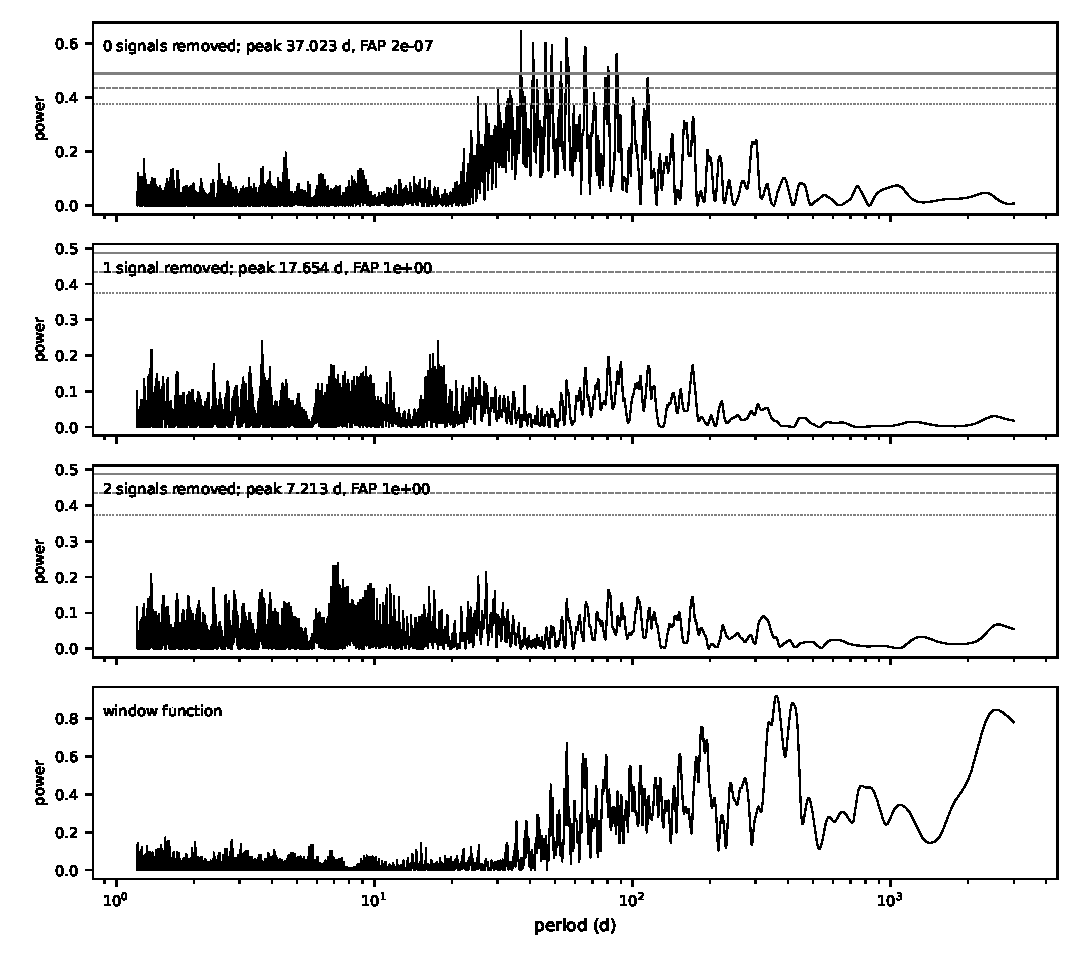
\includegraphics[width=0.92\textwidth]{periodograms.pdf}
\caption{Generalised Lomb-Scargle periodograms of SERVAL's nightly velocities of HD\,125881, each with
the sinusoids of the signals above it fitted jointly, and the observing window's spectral window at the
bottom. The horizontal lines are the false-alarm levels of 0.1, 0.01 and 0.001.}\label{fig:periodograms}
\end{figure}

\subsection{Models}

Models with no planet, with the planet and with a second one at the residuals' highest peak were fitted
by least squares, each with an offset and a jitter added to the errors (Table~\ref{tab:models}). The
planet lowers the Bayesian information criterion~\cite{Schwarz1978} by 42.1 with a circular orbit. A
free eccentricity improves the log-likelihood by 3.8 for two more parameters and raises the BIC by 0.4,
so the circular orbit is preferred. A second signal at 17.7\,d lowers the BIC by a further 2.7, which
does not support it.

\begin{table}[!htbp]
\centering
\caption{Models of SERVAL's velocities of HD\,125881: log-likelihood with free and with circular
orbits, the Bayesian information criterion of each, and the free model's jitter and residual scatter.}
\label{tab:models}
\small
\begin{tabular}{l r r r r r r}
\toprule
Periods & $\ln L$ & $\ln L$ (circular) & BIC & BIC (circular) & Jitter (\ms) & Scatter (\ms) \\
\midrule
None & $-157.4$ & $-157.4$ & 322.6 & 322.6 & 4.93 & 4.99 \\
37.0\,d & $-126.6$ & $-130.4$ & 280.9 & 280.5 & 2.65 & 2.77 \\
37.0 and 17.7\,d & $-115.3$ & $-123.1$ & 278.0 & 277.8 & 2.08 & 2.23 \\
\bottomrule
\end{tabular}
\end{table}

\subsection{The month of 2013 and the earlier nights}\label{sec:month}

The 27 nights from 2013 April 3 to May 3 cover 30 days, less than the period. Within them the
velocities vary smoothly, and their own periodogram peaks at 44.7\,d, beyond the run's length, at a
false-alarm level of $1.5\times10^{-9}$: the run holds most of one cycle, which fixes the signal's
amplitude and phase but not its period. The 25 nights of 2004 to 2012 fix the period. Their own
periodogram has no significant peak, its highest at 4.5\,d standing at a false-alarm level of 0.98 and
its power near 37\,d at 1.0. Fitted with the orbit's period and phase held, they give a semi-amplitude
of $4.9 \pm 1.0$\,\ms, against $6.3 \pm 0.8$\,\ms\ from the month of 2013 alone, and the first half of
the nights, these 25 and the first night of 2013, gives the same phase as the second to within
$12 \pm 13^\circ$ (Section~\ref{sec:tests}).

\subsection{Aliases}

A star observed in the same months each year has its signals' aliases at $|1/P \pm 1/\mathrm{yr}|$,
here at 33.6 and 41.2\,d (the daily aliases lie near one day, below the periods searched). They carry
0.430 and 0.608 of the periodogram's power against 0.648 at 37.0\,d, and the circular model refitted
with the planet at either loses 12.6 and 2.9 in log-likelihood. The observing window decides as
well~\cite{Dawson2010}. Three hundred sets of velocities drawn at the observed times from the circular
model with the fitted jitter, with the planet at 37.0\,d, give a ratio of the powers at 37.0 and
33.6\,d of $1.24^{+0.13}_{-0.11}$, and 3 per cent of them reach the observed 1.51; three hundred with
the planet at 33.6\,d give $0.79 \pm 0.08$, and none reaches it. Against 41.2\,d the observed ratio,
1.065, lies at the 5th percentile of the simulations with the planet at 37.0\,d, $1.27 \pm 0.13$, and
above all but one of the three hundred with the planet at 41.2\,d, $0.80 \pm 0.08$. The period is most
likely 37.0\,d; the 41.2-day alias is disfavoured, by a likelihood ratio of 18 and by the window's
simulations, but not excluded.

\section{The instrument and stellar activity}\label{sec:tests}

\subsection{Three reductions}

Table~\ref{tab:reductions} gives the signal in each of the three reductions, with its semi-amplitude
fitted to the first and to the second half of the nights apart; the halves divide the nights at 2013
April 3, so the first holds the 25 earlier nights and the first night of 2013, and the second the rest
of the month of 2013. SERVAL fits a template to every spectrum's whole extracted orders, the pipeline
cross-correlates a binary mask, and the line-by-line velocities weigh each line by its own scatter, so
a signal one reduction made would not stand in the others. The signal stands in all three as the
highest peak of the periodogram and keeps its amplitude and phase from one half to the other in each.

\begin{table}[!htbp]
\centering
\caption{The 37-day signal of HD\,125881 in three reductions of its HARPS spectra: the periodogram's
highest peak, its false-alarm level, and the semi-amplitude in the first and second half of the
nights.}\label{tab:reductions}
\begin{tabular}{l r r r r}
\toprule
Reduction & Nights & Peak (d) & False alarm & $K$ in each half (\ms) \\
\midrule
SERVAL & 52 & 37.03 & $1.8\times10^{-7}$ & $5.33 \pm 0.99$, $6.01 \pm 0.77$ \\
Pipeline & 52 & 37.01 & $2.9\times10^{-7}$ & $5.34 \pm 0.96$, $5.65 \pm 0.78$ \\
Line-by-line, all lines & 52 & 37.03 & $7.8\times10^{-6}$ & $5.32 \pm 1.04$, $5.63 \pm 0.84$ \\
Line-by-line, quiet lines & 52 & 37.03 & $6.1\times10^{-6}$ & $5.34 \pm 1.03$, $5.65 \pm 0.84$ \\
\bottomrule
\end{tabular}
\end{table}

\subsection{Activity indicators}

The periodograms of the chromatic index, the differential line width, the H$\alpha$ and Na\,D indices
and the pipeline's line width and bisector have no power at 37\,d: within 5 per cent of it, each one's
highest peak stands at a false-alarm level of 1.0, and the S index's from DACE's spectra and from the
line-by-line spectra at 0.40 and 0.11. Their own highest peaks lie near a year (the pipeline's line
width at 345\,d, $2\times10^{-7}$, its bisector at 359\,d, $9\times10^{-9}$, and the differential line
width at 340\,d, 0.01), at 617\,d (Na\,D, $4\times10^{-3}$), at 926 and 977\,d (the two S indices,
$7\times10^{-6}$ and $10^{-4}$, a magnetic cycle of a few years) and nowhere significant (the chromatic
index and H$\alpha$).

The S index measured on the same nights follows the orbit's phase, with a correlation of $r = 0.37$
($p = 0.006$), and the residuals after the orbit do not ($r = 0.16$, $p = 0.25$). Fitted beside the
orbit, the S index takes a coefficient of $0.5 \pm 0.5$\,\ms\ per standard deviation and leaves a
semi-amplitude of 5.5\,\ms, against 5.7\,\ms\ without it. With its slow variation taken out, the S
index has no power at 37\,d (a false-alarm level of 1.0). Within the month of 2013 it varies at
14.3\,d at a false-alarm level of $3\times10^{-5}$, the star's rotation, which the velocities do not
follow: their residuals' highest peak lies at 17.7\,d at a false-alarm level of 1.0. The 37-day period
lies far from the rotation and from twice it.

\section{Orbit and mass}\label{sec:orbit}

Table~\ref{tab:orbit} gives the orbit, sampled with emcee~\cite{ForemanMackey2013} and its
differential-evolution moves~\cite{terBraak2006} from the 52 nights, 48 walkers over 20\,000 steps,
with an offset and a jitter and the orbit held circular. Sampled with its eccentricity free, the orbit
keeps its period and semi-amplitude within their errors, and the eccentricity, $0.23^{+0.09}_{-0.10}$,
lies below 0.38 at 95 per cent; a median above zero is what noise gives a quantity that cannot be
negative~\cite{Lucy1971}. Figure~\ref{fig:phased} shows the velocities phased at the period.

\begin{table}[!htbp]
\centering
\caption{HD\,125881\,b: medians and 68 per cent intervals of the circular orbit sampled from the HARPS
velocities, with the star's mass of 1.02\,\Msun; the eccentricity's bound is from the orbit sampled
with it free.}
\label{tab:orbit}
\begin{tabular}{l r}
\toprule
Parameter & Value \\
\midrule
Period (d) & $37.018 \pm 0.024$ \\
Semi-amplitude $K$ (\ms) & $5.66 \pm 0.59$ \\
Time of conjunction (BJD) & $2456398.58 \pm 0.72$ \\
Eccentricity & $< 0.38$ (95 per cent) \\
Minimum mass $m \sin i$ (\Mearth) & $29.8 \pm 3.1$ \\
Semi-major axis (au) & 0.219 \\
Insolation (Earth's) & 28.6 \\
Equilibrium temperature, no albedo (K) & 644 \\
Transit probability & 2.4 per cent \\
Jitter (\ms) & $3.01^{+0.33}_{-0.29}$ \\
\bottomrule
\end{tabular}
\end{table}

\begin{figure}[!htbp]
\centering
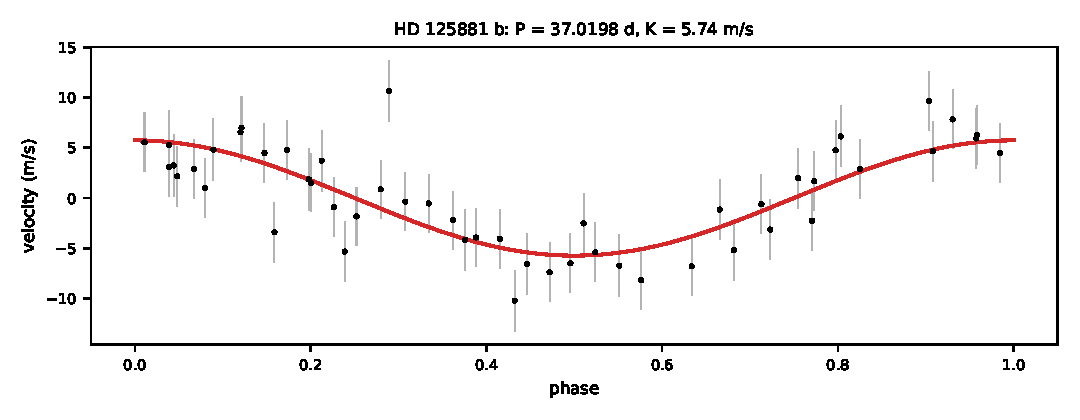
\includegraphics[width=0.95\textwidth]{phased.pdf}
\caption{SERVAL's nightly velocities of HD\,125881 phased at 37.02\,d with the circular orbit. The error
bars include the jitter.}\label{fig:phased}
\end{figure}

The residuals of the circular orbit bound what else the velocities hold (Figure~\ref{fig:limits}). A
circular orbit is recovered 90 per cent of the time at a semi-amplitude of 5.3 to 8.9\,\ms\ at every
period from 1.5 to 90\,d except near 5.9\,d, where it needs 15\,\ms: a minimum mass of 10 to
21\,\Mearth\ out to 16\,d and of 24 to 56\,\Mearth\ from 19 to 90\,d. From 100 to 1\,400\,d it lies at
6.9 to 11.6\,\ms, 59 to 168\,\Mearth, and near 196\,d and from 1\,670 to 2\,470\,d no semi-amplitude
up to 15\,\ms\ is recovered 90 per cent of the time.

\begin{figure}[!htbp]
\centering
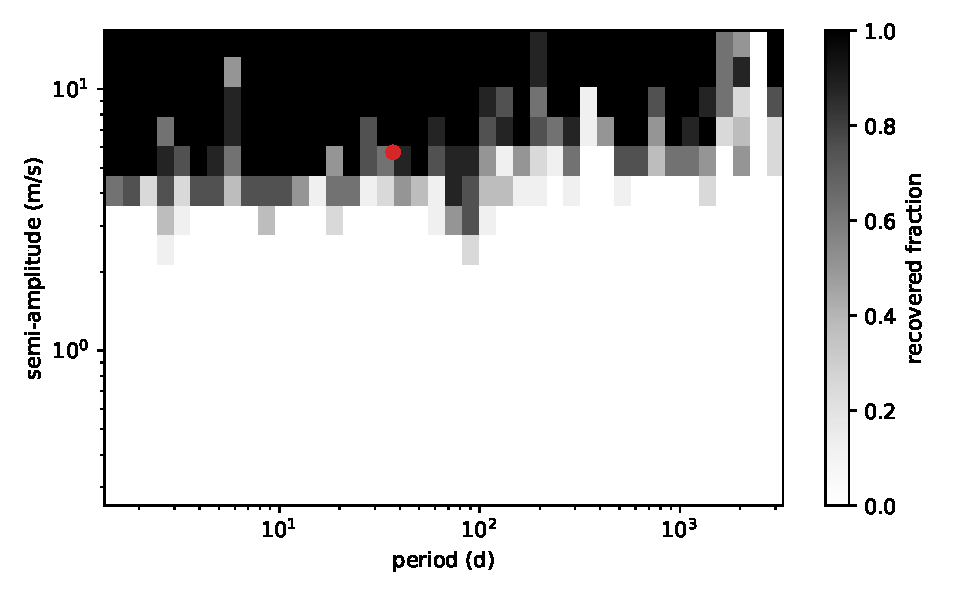
\includegraphics[width=0.8\textwidth]{detection_limits.pdf}
\caption{The fraction of circular orbits injected into the residuals of HD\,125881's velocities that are
recovered, the highest peak of the residual periodogram within 2 per cent of the injected period at a
false-alarm level below $10^{-3}$, eight phases at each period and semi-amplitude. The planet is
marked.}\label{fig:limits}
\end{figure}

\section{TESS}\label{sec:tess}

TESS observed HD\,125881 in six sectors. In four of them the light curve's highest periodogram peak
lies at 0.96\,d, with a semi-amplitude of 86 to 337\,ppm that changes from sector to sector, and in
sectors 65 and 101 at 4.5 and 4.8\,d, at 163 and 193\,ppm. A quiet G dwarf turning in two weeks does
not vary at 0.96\,d; two stars that Gaia flags as variable, of $G = 10.3$ and 13.6, lie about 50\,arcsec
away, two to three of TESS's pixels. Box least squares~\cite{Kovacs2002} within 2 per cent of the
period finds its best box at 36.39\,d, off the orbit's period, and none of its five events lies within
11 days of a predicted conjunction.

The circular orbit's conjunctions, where a transit would fall, carried into the sectors with their
errors, fall in five of them (Table~\ref{tab:tess}). The conjunction of 2019 May 16 lies within sector
11 entirely. There the deepest box of a central transit's length, 6.8\,h, is 497\,ppm deep, at the
level of the light curve's variability in that sector, and a central transit deeper than 718\,ppm, a
planet larger than 3.3 Earth radii, is excluded at $3\sigma$ wherever it falls in the window; a planet
of Neptune's radius would take about 1\,000\,ppm. The conjunction of 2021 May 25 falls at the end of
sector 38, which covers 61 per cent of its probability, and that of 2026 February 28 across the end of
sector 100 and the start of sector 101, which cover 92 per cent of it together.
Table~\ref{tab:conjunctions} gives the conjunctions of the coming year, those of 2027 April to June
when the star stands farthest from the Sun.

\begin{table}[!htbp]
\centering
\caption{The predicted conjunctions of HD\,125881\,b that fall in TESS's sectors, from the circular
orbit: the share of each conjunction's probability the sector covers, the deepest box of a central
transit's length (6.8\,h), and the depth and planet radius above which a central transit is excluded at
$3\sigma$ in the covered part.}\label{tab:tess}
\small
\begin{tabular}{c l r r r r}
\toprule
Sector & Conjunction & Covered & Deepest box (ppm) & Limit (ppm) & Radius (R$_\oplus$) \\
\midrule
11 & 2019 May 16 $\pm$ 1.6\,d & 1.00 & 497 & 718 & 3.3 \\
38 & 2021 May 25 $\pm$ 2.0\,d & 0.61 & 165 & 237 & 1.9 \\
65 & 2023 Jun 5 $\pm$ 2.5\,d & 0.07 & 138 & 277 & 2.0 \\
100 & 2026 Feb 28 $\pm$ 3.1\,d & 0.57 & 574 & 822 & 3.5 \\
101 & 2026 Feb 28 $\pm$ 3.1\,d & 0.35 & 247 & 491 & 2.7 \\
\bottomrule
\end{tabular}
\end{table}

\begin{table}[!htbp]
\centering
\caption{The coming conjunctions of HD\,125881\,b from the circular orbit, with their errors, and the
Sun's distance from the star on each date.}\label{tab:conjunctions}
\begin{tabular}{r l r r}
\toprule
BJD & Date & Error (d) & Solar elongation \\
\midrule
2461470.0 & 2027 Mar 5 & 3.3 & $101^\circ$ \\
2461507.0 & 2027 Apr 11 & 3.3 & $123^\circ$ \\
2461544.1 & 2027 May 18 & 3.4 & $134^\circ$ \\
2461581.1 & 2027 Jun 24 & 3.4 & $125^\circ$ \\
2461618.1 & 2027 Jul 31 & 3.4 & $105^\circ$ \\
\bottomrule
\end{tabular}
\end{table}

\section{Discussion}\label{sec:discussion}

HD\,125881\,b's minimum mass, $29.8 \pm 3.1$\,\Mearth, lies between Neptune's 17 and Saturn's 95. At
0.219\,au from a star of 1.37\,\Lsun\ it would receive 29 times the Earth's insolation, for an
equilibrium temperature of 640\,K with no albedo. The signal stands in three reductions of the same
spectra and has no counterpart at its period in any activity indicator. Its period comes from the 25 nights of 2004 to 2012, which hold the
signal at the orbit's phase at $4.9 \pm 1.0$\,\ms\ but do not find it alone, while 27 nights within one
month, shorter than the period, carry most of its weight, and its one-year alias at 41.2\,d is
disfavoured rather than excluded. Twenty nights of velocities as precise as HARPS's, spread over two or
three months, would decide between 37.0 and 41.2\,d and confirm the planet.

\section{Conclusion}\label{sec:conclusion}

HD\,125881, a quiet G2 dwarf of 1.02\,\Msun\ at 36.2\,pc, carries a Keplerian signal at 37.02\,d and
5.7\,\ms\ in 52 nights of public HARPS velocities, which a planet of at least 30\,\Mearth\ at 0.22\,au
would make. The signal stands in three reductions of the spectra and has no counterpart in eight
activity indicators; most of its weight lies in one month of 2013, and
the earlier nights, which fix its period, agree with it at $4.9 \pm 1.0$\,\ms. New velocities would
confirm it and close the 41.2-day alias, and photometry at the predicted conjunctions would tell
whether it transits.

\section*{Acknowledgements}

Based on data obtained from the ESO Science Archive Facility, on HARPS-RVBank, and on DACE, the Data \&
Analysis Center for Exoplanets, a facility of the University of Geneva and a platform of the Swiss
National Centre of Competence in Research PlanetS. This work has made use of data from the European Space
Agency missions Gaia, processed by the Gaia Data Processing and Analysis Consortium, funded by national
institutions, in particular the institutions participating in the Gaia Multilateral Agreement, and
Hipparcos; and of the TESS mission, funded by NASA's Science Mission Directorate. The velocities, tests
and orbits were computed with orbitlight's planets mode.

\begin{thebibliography}{99}\small\raggedright
\setlength{\itemsep}{1pt}

\bibitem{Howard2010}
A.~W. Howard et al., The occurrence and mass distribution of close-in super-Earths, Neptunes, and
Jupiters, \emph{Science} \textbf{330}, 653 (2010).

\bibitem{Trifonov2020}
T.~Trifonov et al., Public HARPS radial velocity database corrected for systematic errors,
\emph{Astron. Astrophys.} \textbf{636}, A74 (2020).

\bibitem{Zechmeister2018}
M.~Zechmeister et al., Spectrum radial velocity analyser (SERVAL). High-precision radial velocities and
two alternative spectral indicators, \emph{Astron. Astrophys.} \textbf{609}, A12 (2018).

\bibitem{LoCurto2015}
G.~Lo Curto et al., HARPS gets new fibres after 12 years of operations, \emph{The Messenger}
\textbf{162}, 9 (2015).

\bibitem{Bouchy2001}
F.~Bouchy, F.~Pepe and D.~Queloz, Fundamental photon noise limit to radial velocity measurements,
\emph{Astron. Astrophys.} \textbf{374}, 733 (2001).

\bibitem{Artigau2022}
\'E.~Artigau et al., Line-by-line velocity measurements: an outlier-resistant method for precision
velocimetry, \emph{Astron. J.} \textbf{164}, 84 (2022).

\bibitem{Ricker2015}
G.~R. Ricker et al., Transiting Exoplanet Survey Satellite, \emph{J. Astron. Telesc. Instrum. Syst.}
\textbf{1}, 014003 (2015).

\bibitem{Lightkurve2018}
Lightkurve Collaboration, Lightkurve: Kepler and TESS time series analysis in Python, Astrophysics
Source Code Library, ascl:1812.013 (2018).

\bibitem{GaiaDR3}
Gaia Collaboration, A.~Vallenari et al., Gaia Data Release 3. Summary of the content and survey
properties, \emph{Astron. Astrophys.} \textbf{674}, A1 (2023).

\bibitem{Creevey2023}
O.~L. Creevey et al., Gaia Data Release 3. Astrophysical parameters inference system (Apsis). I. Methods
and content overview, \emph{Astron. Astrophys.} \textbf{674}, A26 (2023).

\bibitem{Perryman1997}
M.~A.~C. Perryman et al., The Hipparcos catalogue, \emph{Astron. Astrophys.} \textbf{323}, L49 (1997).

\bibitem{Noyes1984}
R.~W. Noyes et al., Rotation, convection, and magnetic activity in lower main-sequence stars,
\emph{Astrophys. J.} \textbf{279}, 763 (1984).

\bibitem{Mamajek2008}
E.~E. Mamajek and L.~A. Hillenbrand, Improved age estimation for solar-type dwarfs using
activity-rotation diagnostics, \emph{Astrophys. J.} \textbf{687}, 1264 (2008).

\bibitem{Zechmeister2009}
M.~Zechmeister and M.~K\"urster, The generalised Lomb-Scargle periodogram. A new formalism for the
floating-mean and Keplerian periodograms, \emph{Astron. Astrophys.} \textbf{496}, 577 (2009).

\bibitem{Baluev2008}
R.~V. Baluev, Assessing the statistical significance of periodogram peaks, \emph{Mon. Not. R. Astron.
Soc.} \textbf{385}, 1279 (2008).

\bibitem{Schwarz1978}
G.~Schwarz, Estimating the dimension of a model, \emph{Ann. Statist.} \textbf{6}, 461 (1978).

\bibitem{Dawson2010}
R.~I. Dawson and D.~C. Fabrycky, Radial velocity planets de-aliased: a new, short period for super-Earth
55 Cnc e, \emph{Astrophys. J.} \textbf{722}, 937 (2010).

\bibitem{ForemanMackey2013}
D.~Foreman-Mackey, D.~W. Hogg, D.~Lang and J.~Goodman, emcee: the MCMC hammer, \emph{Publ. Astron. Soc.
Pac.} \textbf{125}, 306 (2013).

\bibitem{terBraak2006}
C.~J.~F. ter Braak, A Markov chain Monte Carlo version of the genetic algorithm Differential Evolution:
easy Bayesian computing for real parameter spaces, \emph{Stat. Comput.} \textbf{16}, 239 (2006).

\bibitem{Lucy1971}
L.~B. Lucy and M.~A. Sweeney, Spectroscopic binaries with circular orbits, \emph{Astron. J.}
\textbf{76}, 544 (1971).

\bibitem{Kovacs2002}
G.~Kov\'acs, S.~Zucker and T.~Mazeh, A box-fitting algorithm in the search for periodic transits,
\emph{Astron. Astrophys.} \textbf{391}, 369 (2002).

\end{thebibliography}

\end{document}
